\documentclass{article}

\usepackage{amsmath}
\usepackage{amssymb}
\usepackage{longtable}
\usepackage{courier}
\usepackage{indentfirst}
\usepackage{booktabs}
\usepackage{graphicx} 
\usepackage{float}

%\renewcommand\thetable{\arabic{section}.\arabic{subsection}.\arabic{table}}
%\renewcommand\thefigure{\arabic{section}.\arabic{subsection}.\arabic{table}}

\input{PToP-macro}

\allowdisplaybreaks[4]

\title{\LaTeX ML A1}
\author{Zhen}

%\def\row#1{$#1$ & \protect{\verb/xyz/}}
%\newcommand{\row}[1]{$#1$ & xyz}

\begin{document}

\begin{center}
\Huge CSC2515 Assignment \#1 \\ 
\Large Zhen Li, zhen@cs.toronto.edu
\end{center}

\section{Logistic Regression}

\subsection{Bayes' Rule}

\begin{align*}
\Blank & p(y=1 | \mathbf{x}) && \text{Use Bayes' Rule}\\
\Eq & \frac{p(\mathbf{x} | y=1) \cdot p(y=1)}{p(\mathbf{x})}\\
\Eq & \frac{p(\mathbf{x} | y=1) \cdot p(y=1)}{p(\mathbf{x} | y=1) \cdot p(y=1) + p(\mathbf{x} | y=0) \cdot p(y=0)}\\
\Eq & \frac{1}{1 + \dfrac{p(\mathbf{x} | y=0) \cdot p(y=0)}{p(\mathbf{x} | y=1) \cdot p(y=1)}}\\
\Eq & \frac{1}{1 + \dfrac{\prod_{i=1}^{D} p(x_i | y=0) \cdot (1-\alpha)}{\prod_{i=1}^{D} p(x_i | y=1) \cdot \alpha}}\\
\Eq & \frac{1}{1 + \dfrac{\prod_{i=1}^{D} \dfrac{1}{\sqrt{2\pi}\sigma_i} \exp\{-\dfrac{1}{2\sigma_i^2} (x_i-\mu_{i0})^2\} \cdot (1-\alpha)}{\prod_{i=1}^{D} \dfrac{1}{\sqrt{2\pi}\sigma_i} \exp\{-\dfrac{1}{2\sigma_i^2} (x_i-\mu_{i1})^2\} \cdot \alpha}}\\
\Eq & \frac{1}{1 + \prod_{i=1}^{D} \dfrac{\exp\{-\dfrac{1}{2\sigma_i^2} (x_i-\mu_{i0})^2\}}{\exp\{-\dfrac{1}{2\sigma_i^2} (x_i-\mu_{i1})^2\}} \cdot \dfrac{(1-\alpha)}{\alpha}}\\
\Eq & \frac{1}{1 + \prod_{i=1}^{D} \exp\{-\dfrac{1}{2\sigma_i^2} ( (x_i-\mu_{i0})^2 - (x_i-\mu_{i1})^2 )\} \cdot \dfrac{(1-\alpha)}{\alpha}}\\
\Eq & \frac{1}{1 + \prod_{i=1}^{D} \exp\{-\dfrac{1}{2\sigma_i^2} ( (x_i-\mu_{i0})^2 - (x_i-\mu_{i1})^2 )\} \cdot \dfrac{(1-\alpha)}{\alpha}}\\
\Eq & \frac{1}{1 + \prod_{i=1}^{D} \exp\{-\dfrac{1}{2\sigma_i^2} ( -2(\mu_{i0} - \mu_{i1})x_i + (\mu_{i0}^2 - \mu_{i1}^2) )\} \cdot \dfrac{(1-\alpha)}{\alpha}}\\
\Eq & \frac{1}{1 + \exp\{ \sum_{i=1}^{D}  ( \dfrac{\mu_{i0} - \mu_{i1}}{\sigma_i^2} \cdot x_i - \dfrac{\mu_{i0}^2 - \mu_{i1}^2}{2\sigma_i^2} ) \} \cdot \exp\{ \ln\dfrac{(1-\alpha)}{\alpha} \}  }
\end{align*}

Comparing with the given format
\begin{align*}
p(y=1 | \mathbf{x}) \Eq \sigma(\mathbf{w}^{T}\mathbf{x}+b) \Eq \frac{1}{1 + \exp(-\sum_{i=1}^{D} w_{i}x_{i}-b)}
\end{align*}

And hence we have
\begin{align*}
w_i \Eq & \dfrac{\mu_{i1} - \mu_{i0}}{\sigma_i^2} \\
b \Eq & \sum_{i=1}^{D}  \dfrac{\mu_{i0}^2 - \mu_{i1}^2}{2\sigma_i^2} - \ln\dfrac{(1-\alpha)}{\alpha}\\
\end{align*}

\subsection{Maximum Likelihood Estimation}

\ \\

From the given format of $p(y=1| \mathbf{x}^{(n)}, \mathbf{w}, b)$, we can derive $p(y=0| \mathbf{x}^{(n)}, \mathbf{w}, b)$
\begin{align*}
p(y=1| \mathbf{x}^{(n)}, \mathbf{w}, b) & \Eq \sigma(\mathbf{w}^{T}\mathbf{x}^{(n)} + b) \Eq \frac{1}{1 + \exp(-\sum_{i=1}^{D} w_{i}x_{i}^{(n)} - b)}\\
p(y=0| \mathbf{x}^{(n)}, \mathbf{w}, b) & \Eq 1 - p(y=1| \mathbf{x}^{(n)}, \mathbf{w}, b) \Eq \frac{\exp(-\sum_{i=1}^{D} w_{i}x_{i}^{(n)} - b)}{1 + \exp(-\sum_{i=1}^{D} w_{i}x_{i}^{(n)} - b)}\\
\Blank \text{To simplify, let } & k = \exp(-\sum_{i=1}^{D} w_{i}x_{i}^{(n)} - b) \text{, and hence we have}\\
p(y=1| \mathbf{x}^{(n)}, \mathbf{w}, b) & \Eq \frac{1}{1 + k}\\
p(y=0| \mathbf{x}^{(n)}, \mathbf{w}, b) & \Eq \frac{k}{1 + k}
\end{align*}

Thus the likelihood function is
\begin{align*}
\Blank & p(\mathbf{y} | \mathbf{x}, \mathbf{w}, b)\\
\Eq & \prod_{n=1}^{N} [p(y=0 | \mathbf{x}^{(n)}, \mathbf{w}, b)]^{1-y^{(n)}} [p(y=1| \mathbf{x}^{(n)}, \mathbf{w}, b)]^{y^{(n)}}\\
\Eq & \prod_{n=1}^{N} (\frac{k}{1 + k})^{1-y^{(n)}} (\frac{1}{1 + k})^{y^{(n)}}
\end{align*}

Then the negative log-likelihood expression is
\begin{align*}
\Blank & E(\mathbf{w}, b)\\
\Eq & -\ln\{ p(\mathbf{y} | \mathbf{x}, \mathbf{w}, b) \}\\
\Eq & -\sum_{n=1}^{N} \{ (1-y^{(n)}) [\ln(k) - \ln(1 + k)] + y^{(n)} [-\ln(1 + k)] \}\\
\Eq & \sum_{n=1}^{N} \{ (y^{(n)}-1)\ln(k) + \ln(1 + k) \} && \text{replace } k\\
\Eq & \sum_{n=1}^{N} \{ (y^{(n)}-1)\ln[\exp(-\sum_{i=1}^{D} w_{i}x_{i}^{(n)} - b)] + \ln[1 + \exp(-\sum_{i=1}^{D} w_{i}x_{i}^{(n)} - b)] \}\\
\Eq & \sum_{n=1}^{N} \{ (y^{(n)}-1)(-\sum_{i=1}^{D} w_{i}x_{i}^{(n)} - b) + \ln[1 + \exp(-\sum_{i=1}^{D} w_{i}x_{i}^{(n)} - b)] \}
\end{align*}

The derivative with respect to $b$
\begin{align*}
\Blank  \frac{\partial E(\mathbf{w}, b)}{\partial b} \Eq  \sum_{n=1}^{N} \{\frac{1}{1 + \exp(- \sum_{i=1}^{D} w_{i}x_{i}^{(n)} - b)} - y^{(n)}\}
\end{align*}

The derivative with respect to $w_i$
\begin{align*}
\Blank  \frac{\partial E(\mathbf{w}, b)}{\partial w_i} \Eq  \sum_{n=1}^{N} \{ x_{i}^{(n)} (\frac{1}{1 + \exp(- \sum_{i=1}^{D} w_{i}x_{i}^{(n)} - b)} - y^{(n)}) \}\\
\end{align*}

\subsection{L2 Regularization}

\ \\

Use Bayes' Rule
\begin{align*}
& p(\mathbf{w}, b | D) \propto p(D | \mathbf{w}, b) p(\mathbf{w}, b)
\end{align*}

Based on the prior and likelihood defined above
\begin{align*}
\Blank & p(D | \mathbf{w}, b) p(\mathbf{w}, b)\\
\Eq & p(D | \mathbf{w}, b) \cdot \prod_{i=1}^{D} p(w_i) \cdot p(b))\\
\Eq & p(D | \mathbf{w}, b) \cdot \prod_{i=1}^{D} \mathcal{N}(w_i | 0, 1/\lambda) \cdot \mathcal{N}(b | 0, 1/\lambda)\\
\Eq & p(D | \mathbf{w}, b) \cdot \prod_{i=1}^{D} ( \sqrt{\frac{\lambda}{2\pi}} \exp(-\frac{\lambda}{2}w_i^2) ) \cdot  \sqrt{\frac{\lambda}{2\pi}} \exp(-\frac{\lambda}{2}b^2)\\
\end{align*}

Define $L(\mathbf{w},b)$ to be the negative logarithm of the expression above
\begin{align*}
\Blank & L(\mathbf{w},b)\\
\Eq & -\ln\{ p(D | \mathbf{w}, b) \cdot \prod_{i=1}^{D} ( \sqrt{\frac{\lambda}{2\pi}} \exp(-\frac{\lambda}{2}w_i^2) ) \cdot  \sqrt{\frac{\lambda}{2\pi}} \exp(-\frac{\lambda}{2}b^2) \}\\
\Eq & -\ln\{ p(D | \mathbf{w}, b) \} -\sum_{i=1}^{D} \{ \frac{1}{2} (\ln \lambda - \ln 2 \pi) - \frac{\lambda}{2}w_i^2 \} - \{ \frac{1}{2} (\ln \lambda - \ln 2 \pi) - \frac{\lambda}{2}b^2 \}\\
\Eq & E(\mathbf{w},b) + \frac{\lambda}{2} \sum_{i=1}^{D} w_i^2 + \frac{\lambda}{2}b^2 + \{ \frac{-(|D| + 1)}{2}(\ln \lambda - \ln 2 \pi) \}
\end{align*}

This matches the given form, where
\begin{align*}
C(\lambda) \Eq \frac{-(|D| + 1)}{2}(\ln \lambda - \ln 2 \pi)
\end{align*}

The derivative with respect to $w_i$, and $b$
\begin{align*}
\iffalse
\frac{\partial L(\mathbf{w},b)}{\partial \lambda} & \Eq \frac{1}{2} \sum_{i=1}^{D} w_i^2 + \frac{b^2}{2} - \frac{|D| + 1}{2 \lambda}\\
\fi
\frac{\partial L(\mathbf{w},b)}{\partial w_i} & \Eq \frac{\partial E(\mathbf{w}, b)}{\partial w_i} + \lambda w_i \Eq \sum_{n=1}^{N} \{ x_{i}^{(n)} (\frac{1}{1 + \exp(- \sum_{i=1}^{D} w_{i}x_{i}^{(n)} - b)} - y^{(n)}) \} + \lambda w_i\\
\frac{\partial L(\mathbf{w},b)}{\partial b} & \Eq \frac{\partial E(\mathbf{w}, b)}{\partial b} + \lambda b \Eq \sum_{n=1}^{N} \{\frac{1}{1 + \exp(- \sum_{i=1}^{D} w_{i}x_{i}^{(n)} - b)} - y^{(n)} \} + \lambda b\\
\end{align*}

\section{Digit Classification}

\subsection{k-Nearest Neighbours}

I run kNN for different $k \in \{1,3,5,7,9\}$ (script: \texttt{calc\_knn.m}), then calculates the classification rate on the validation set(Table \ref{table:knn} and Figure \ref{fig:knn}).\\

\begin{table}[htbp]
\centering
\begin{tabular}{lccccc}
\toprule
k & 1 & 3 & 5 & 7 & 9\\
\midrule
classification rate & 0.82 & 0.86 & 0.86 & 0.86 & 0.84\\
\bottomrule
\end{tabular}
\caption{Experiment result for the 5 values of $k$.
\label{table:knn}}
\end{table} 

\begin{figure}[ht]
\centering
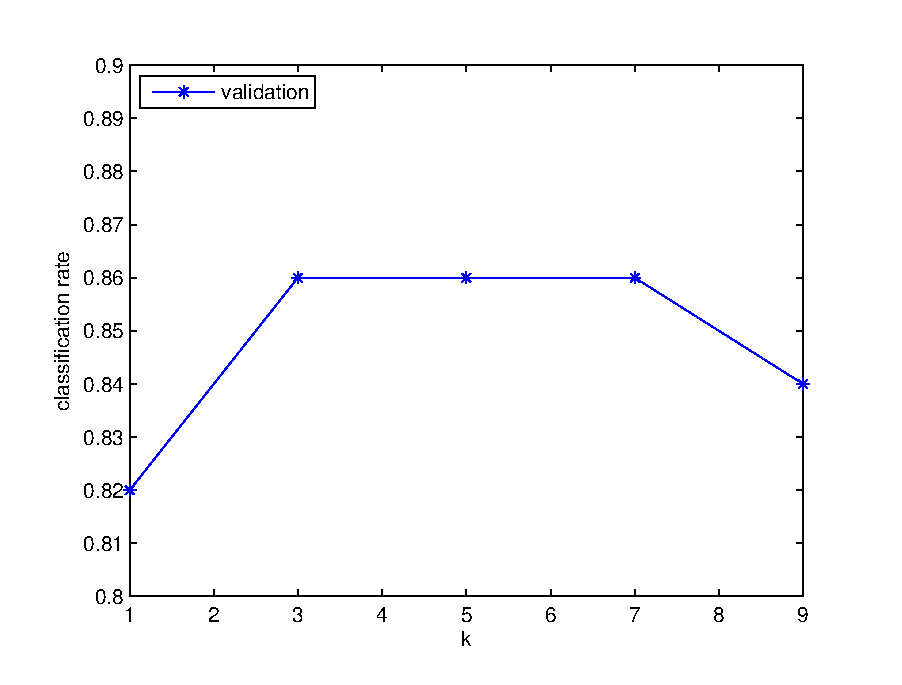
\includegraphics[width=\textwidth]{knn.eps}
\caption{Experiment result for the 5 values of $k$. 
\label{fig:knn}}
\end{figure}

The classification rate is not satisfying, where the highest one is just $0.86$. According to the curve, I chose $k^*=5$, which seems to be at the top of the curve, and tested it using \texttt{mnist\_test}. The classification rate is $0.94$ for $k^*=5$. \\

In addition, I also tested for $k^*+2$ and $k^*-2$(that is, $3$ and $7$), compared the performance with the validation performance(Table \ref{table:kstarnn} and Figure \ref{fig:kstarnn}).\\

\begin{table}[htbp]
\centering
\begin{tabular}{lccccc}
\toprule
k & 1 & 3 & 5 & 7 & 9\\
\midrule
classification rate(validation) & 0.82 & 0.86 & 0.86 & 0.86 & 0.84\\
classification rate(test) & n/a & 0.92 & 0.94 & 0.94 & n/a\\
\bottomrule
\end{tabular}
\caption{Comparison of the classification rate on the validation set and test set of \{ $k^*$, $k^*+2$, and $k^*-2$ \}.
\label{table:kstarnn}}
\end{table} 

\begin{figure}[ht]
\centering
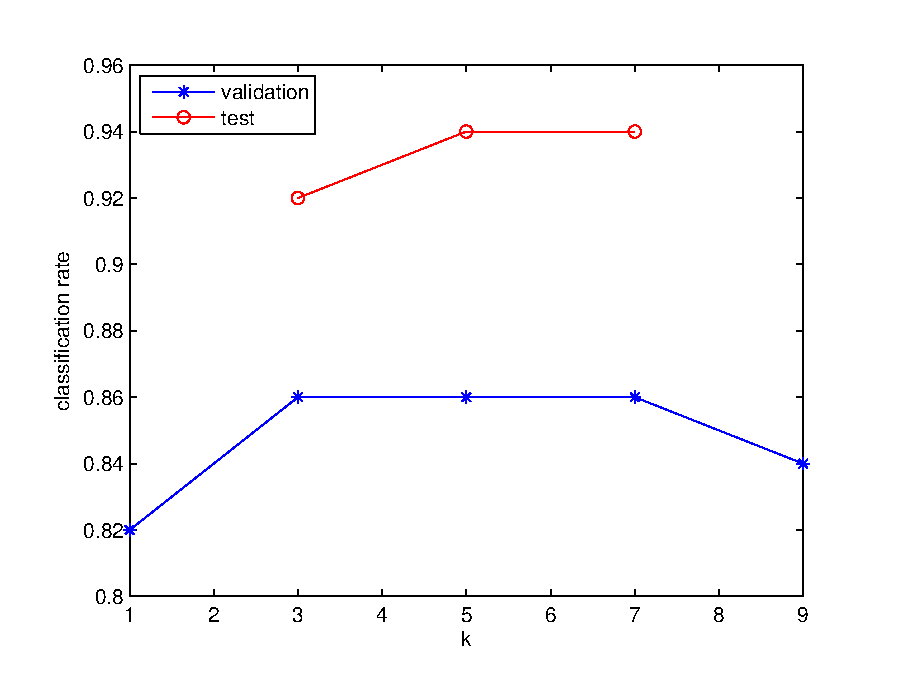
\includegraphics[width=\textwidth]{kstarnn.eps}
\caption{Comparison of the classification rate on the validation set and test set of \{ $k^*$, $k^*+2$, and $k^*-2$ \}. 
\label{fig:kstarnn}}
\end{figure}


We can observe that the test performance for these values of $k$ correspond to the validation performance. \\

However, the performance for different values of $k$ in the validation is not significant. In this problem, I chose $k^* = 5$ and the test performance correspond to the validation performance, and this may be a coincidence. So maybe we need a more complicated and powerful method, or we need to change the Euclidean Distance Function to a regularized one, as suggested in the course slides.\\

\subsection{Logistic Regression}

I implemented a vectorized Matlab script to make it faster. The return value of \texttt{checkgrad} is approximately $10^{-9}$, which is satisfying. I initialized the weights using $0.5 * \texttt{randn}$, a psuedorandom scalar drawn from the standard normal distribution. \\

\begin{table}[htbp]
\centering
\begin{tabular}{lcc|cc|cc}
\toprule
\ & \ & \ & train & \ & validation & \\
id & $learning\_rate$ & $num\_iterations$ & cross\_entropy & error & cross\_entropy & error \\
\midrule
1 & 0.25 & 100 & 12.79  & 0.015 & 16.56 & 0.144\\
2 & 0.25 & 300 & 4.580  & 0 & 14.17 & 0.120\\
3 & 0.25 & 500 & 2.654  & 0 & 9.892 & 0.084\\
4 & 0.50 & 100 & 5.937  & 0 & 12.87 & 0.104\\
5 & 0.50 & 300 & 2.279  & 0 & 13.72 & 0.108\\
6 & 0.50 & 500 & 1.399  & 0 & 12.74 & 0.112\\
7 & 1.0  & 100 & 2.810  & 0 & 15.05 & 0.116\\
8 & 1.0  & 300 & 1.087  & 0 & 14.54 & 0.108\\
9 & 1.0  & 500 & 0.6832 & 0 & 13.74 & 0.104\\
\bottomrule
\end{tabular}
\caption{Cross entropy and classification error on the training and validation sets using different hyperparameter combinations. The average cross entropy and classification error is calculated from 20 re-runs for each condition, in order to reduce the affect of different initial weights. 
\label{table:hyper}}
\end{table} 

\begin{figure}[htbp]
\centering
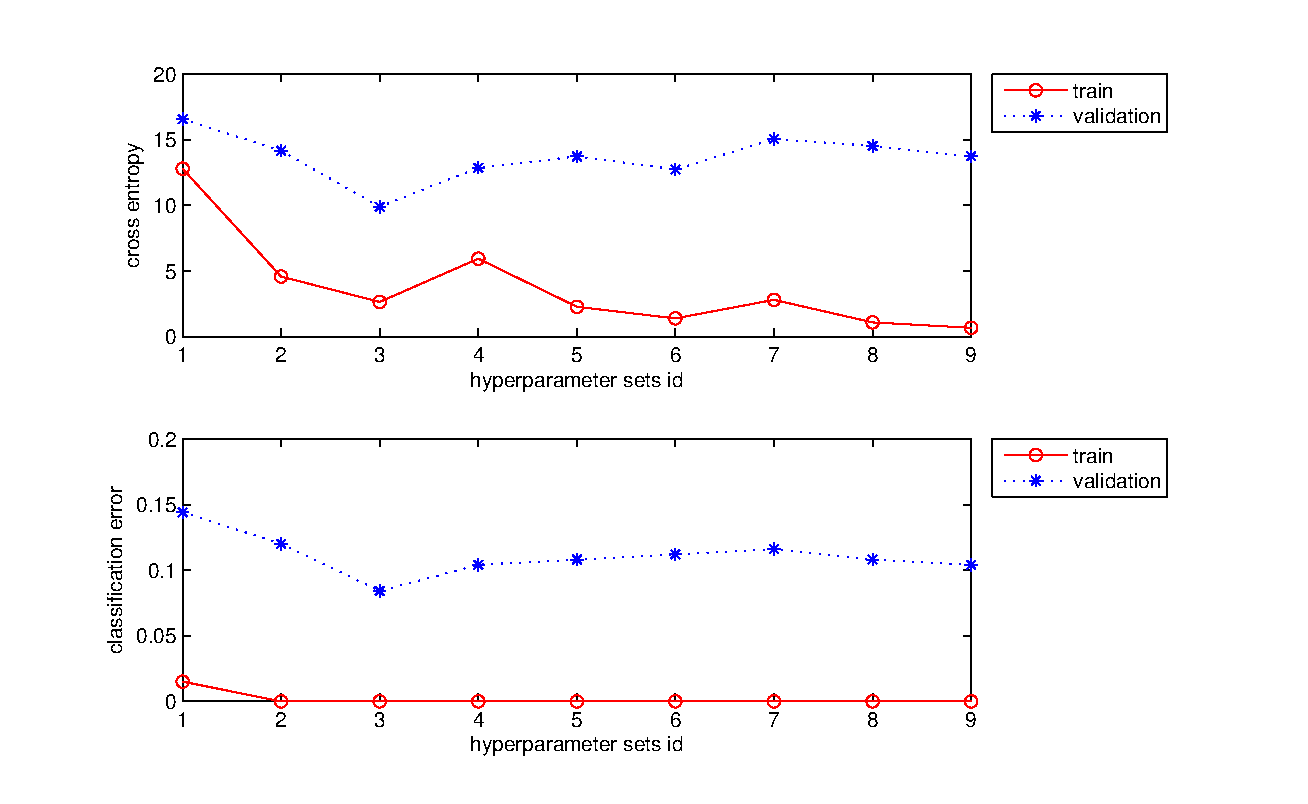
\includegraphics[width=\textwidth]{2-2-findhyper.eps}
\caption{The cross entropy(top plot) and the classification error(bottom plot) on the training and validation sets, using different hyperparameter combination sets. The id is the same as Table \ref{table:hyper}.
\label{fig:findhyper}}
\end{figure}

As for the hyperparameters, I set $learning\_rate=1$ and $num\_iterations=100$ at first. I got some Nan/Inf errors when the $learning\_rate$ gets 2 or bigger. I also tried to set $num\_iterations=500$, and the execution time is just 1 or 2 seconds, which is affordable. So I set different values of the $learning\_rate$ and $num\_iterations$ within this range, and run the logistic regression for 20 times for each hyperparameter set. The average result is shown in Table \ref{table:hyper} and Figure \ref{fig:findhyper}.\\

We can observe that there are no significant differences in classification error of these hyperparameter combinations. Considering that we need the minimum cross entropy and classification error on the validation set, I chose the 3rd combination, in which $learning\_rate=0.25$ and $num\_iterations=500$. Its cross entropy on the validation set is 9.892, while its classification error is 0.084. Then I re-run the code on the test set for 20 times to compare their performance.\\

\begin{table}[htbp]
\centering
\begin{tabular}{lcc}
\toprule
id & cross\_entropy(test) & classification\_error(test) \\
\midrule
1   & 12.95 & 0.080\\
2   & 12.43 & 0.060\\
3   & 18.87 & 0.060\\
4   & 12.41 & 0.080\\
5   & 10.95 & 0.060\\
6-20& ...   & ... \\
\midrule
Average & 13.95 & 0.073\\
\bottomrule
\end{tabular}
\caption{Cross entropy and classification error on the test set when $learning\_rate=0.25$ and $num\_iterations=500$. Test id No.6 to No.20 has been omitted in this table to save the space. 
\label{table:hyper-final}}
\end{table} 

\begin{figure}[htb]
\centering
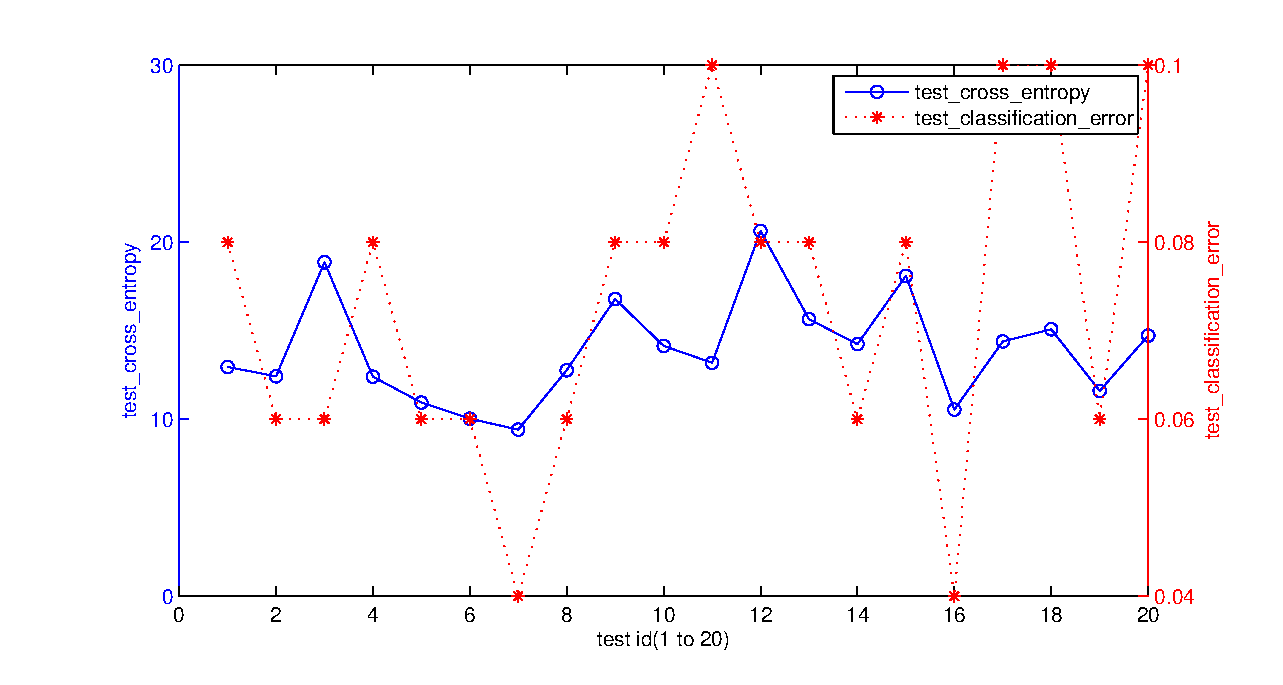
\includegraphics[width=\textwidth]{logistic-test.eps}
\caption{Cross entropy and classification error on the test set when $learning\_rate=0.25$ and $num\_iterations=500$.
\label{fig:logistic-test}}
\end{figure}

I found that the averaged cross entropy on the test set became a little worse (9.892 to 13.95), but the classification error rate has decreased from 0.084 to 0.073. Though it is not perfect, but I think it is satisfying for this simple model.\\

Then let's observe the cross entropy changes as training progresses. I chose the same hyperparameter sets as above, and plotted two graphs for \texttt{mnist\_train} and \texttt{mnist\_train\_small}. Each plot show curves for the training set and validation set. I run my code for 5 times and marked the curves with different colors.\\

\begin{figure}[htb]
\centering
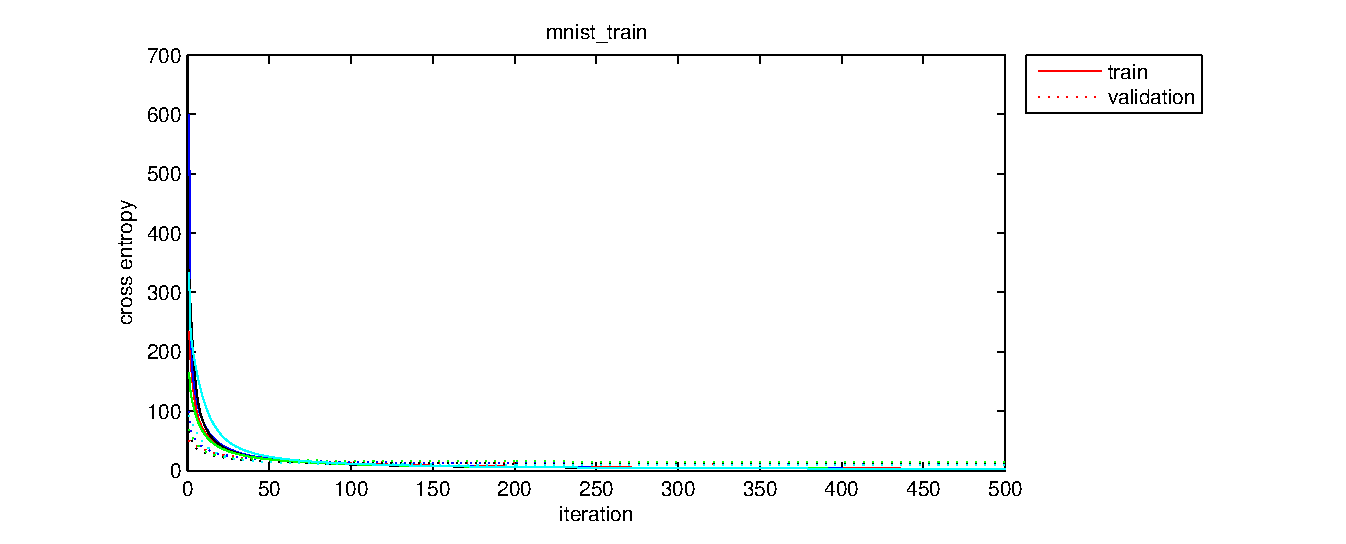
\includegraphics[width=\textwidth]{ce-train.eps}
\caption{The cross entropy for the training set and validation set changes as training progresses.
\label{fig:ce-train}}
\end{figure}

\begin{figure}[htb]
\centering
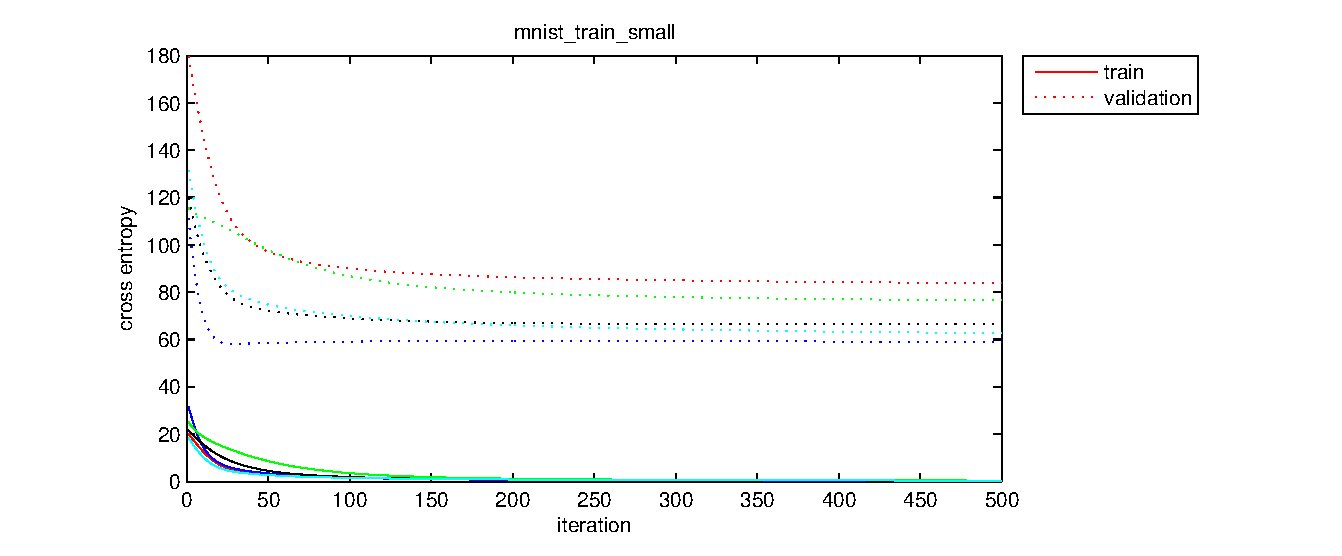
\includegraphics[width=\textwidth]{ce-train-s.eps}
\caption{The cross entropy for the small training set and validation set changes as training progresses.
\label{fig:ce-train-s}}
\end{figure}

From Figure \ref{fig:ce-train} and Figure \ref{fig:ce-train-s}, we have two conclusions. First, we can conclude that the smaller training set leads to worse cross entropy. So we need to get more training data in practical. Second, the results change when we run the code several times. So we need to run multiple times and calculate the average performance to choose the best parameter settings.\\

\subsection{Penalized Logistic Regression}

Similar to section 2.2, I repeated the logistic regression algorithm after verifying my code with the \texttt{checkgrad}. I wrote a script (\texttt{logistic\_regression\_ pen\_template.m}) to validate the different values for $\lambda \in \{0.001, 0.01, 0.1, 1.0\}$. But I found that it is not convincing to explain the cross entropy and classificatio error change on $\lambda$, so I add more values to the set, that is, I run the code with $\lambda \in \{0.001, 0.005, 0.01, 0.05, 0.1, 0.5, 1.0, 2.0\}$. \\

For each $\lambda$, it will re-run 20 times to balance the different initialization of weights. Then the averaged cross entropy and classification error is recorded on the training and validation sets. As required by the assignment, I also trained with the smaller dataset(\texttt{mnist\_train\_small}), and let's compare their performance.\\

\begin{figure}[htb]
\centering
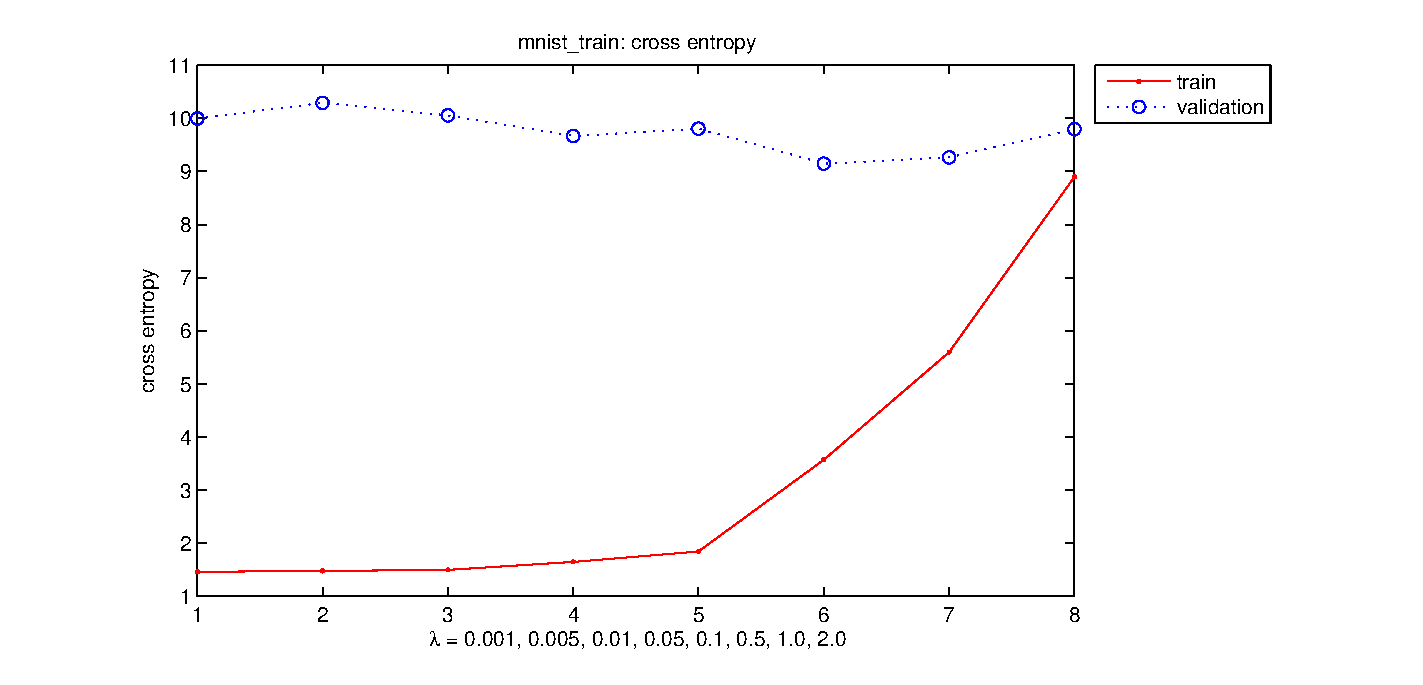
\includegraphics[width=\textwidth,height=5cm]{2-3-train-ce.eps}
\caption{The averaged cross entrop for the training(\texttt{mnist\_train}) and validation(\texttt{mnist\_valid}) sets against $\lambda$.
\label{fig:2-3-train-ce}}
\end{figure}

\begin{figure}[H]
\centering
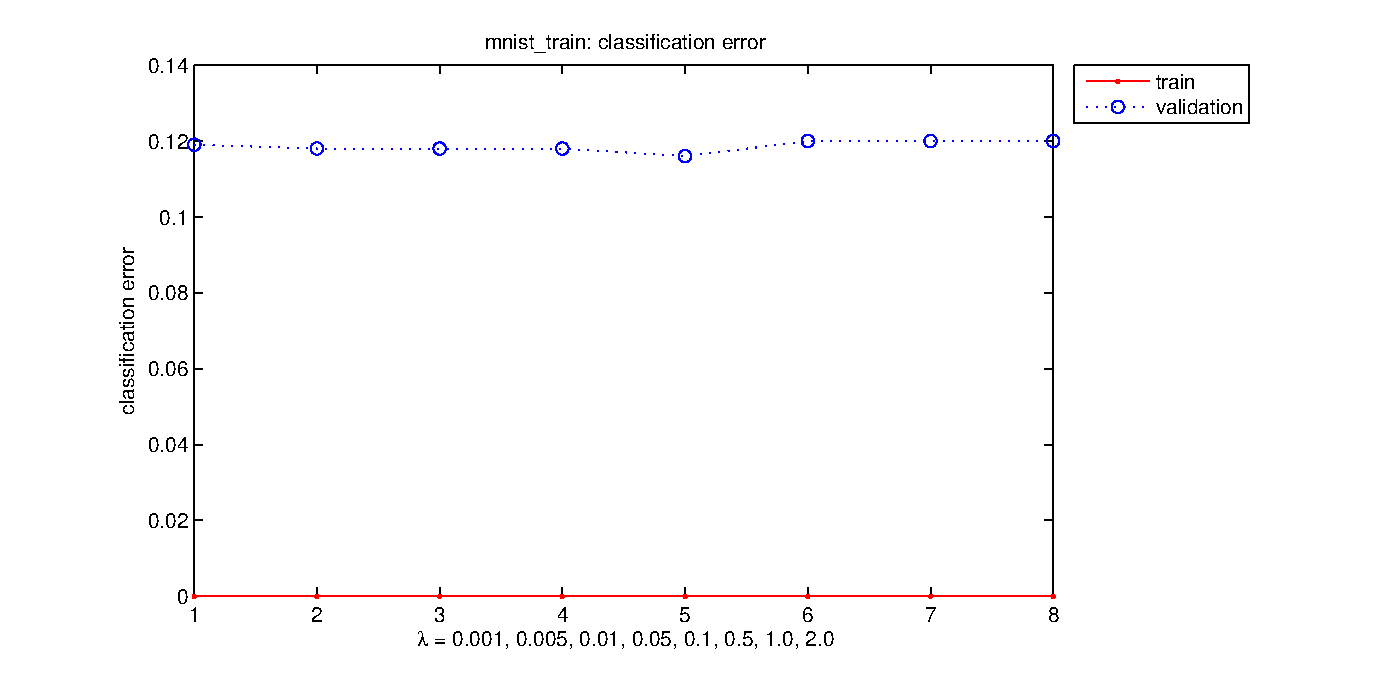
\includegraphics[width=\textwidth,height=5cm]{2-3-train-error.eps}
\caption{The averaged classification error for the training(\texttt{mnist\_train}) and validation(\texttt{mnist\_valid}) sets against $\lambda$.
\label{fig:2-3-train-er}}
\end{figure}

\begin{figure}[H]
\centering
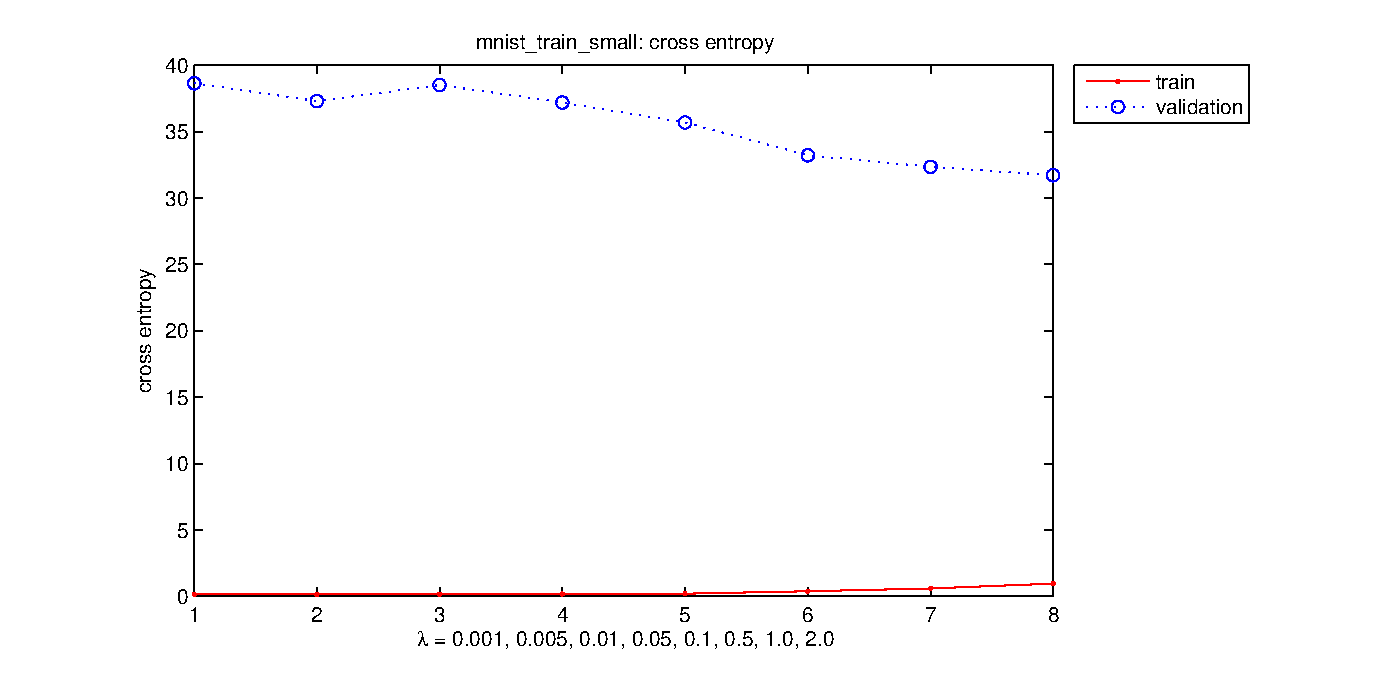
\includegraphics[width=\textwidth,height=5cm]{2-3-train-s-ce.eps}
\caption{The averaged cross entropy for the training(\texttt{mnist\_train\_small}) and validation(\texttt{mnist\_valid}) sets against $\lambda$.
\label{fig:2-3-train-s-ce}}
\end{figure}

\begin{figure}[H]
\centering
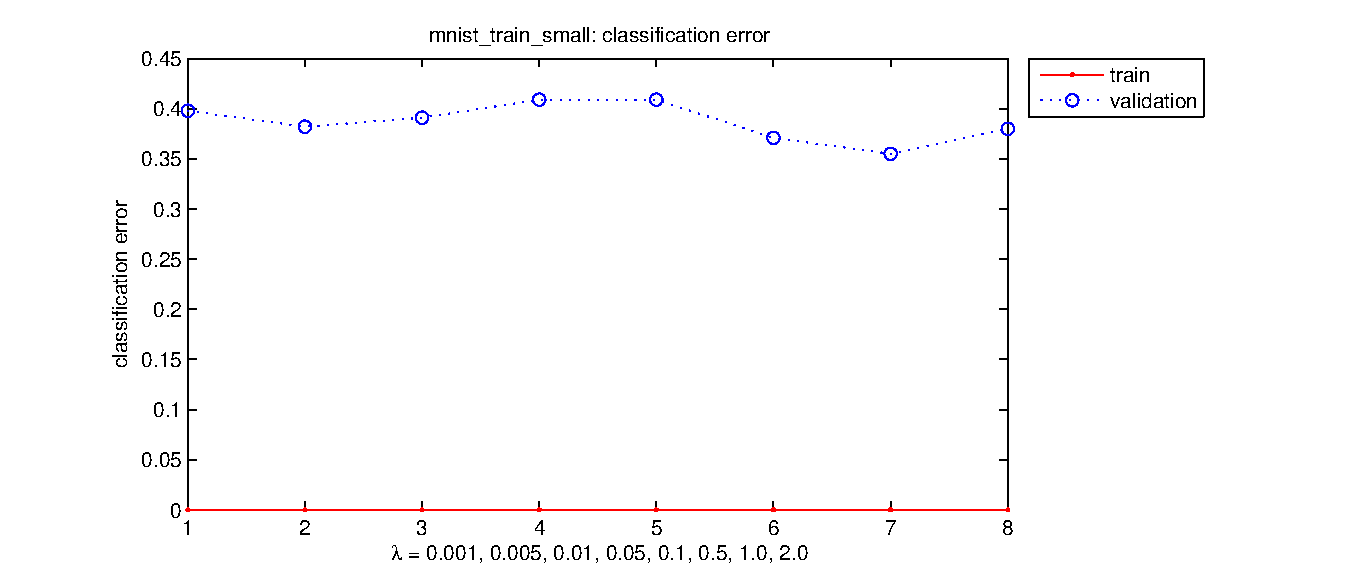
\includegraphics[width=\textwidth,height=5cm]{2-3-train-s-error.eps}
\caption{The averaged classification error for the training(\texttt{mnist\_train\_small}) and validation(\texttt{mnist\_valid}) sets against $\lambda$.
\label{fig:2-3-train-s-er}}
\end{figure}

The regular pattern seems not obvious from these graphs. However, from \texttt{mnist\_train}(Figure \ref{fig:2-3-train-ce} and Figure \ref{fig:2-3-train-er}), we can infer that the cross entropy and classification error on the validation set will get lower(better) with $\lambda=0.5$ or $1$. From the \texttt{mnist\_train\_small}(Figure \ref{fig:2-3-train-s-ce} and Figure \ref{fig:2-3-train-s-er}), we can also infer that the cross entropy and classification error will get lower at around $\lambda=0.5$ or $1$ or $2$.\\

I will go with $\lambda^{*}=0.5$ based on the results from \texttt{mnist\_train}, since we have found that a training set with more samples is more convincing. That means the performance will get better(the curve will go down) at first, before $\lambda^{*}$, then the performance will get worse(the curve will go up).\\

I think one of the reasons is that if $\lambda$ is too big comparing to $\mathbf{w}$, then it will lead to a bad modification for every iteration. As I mentioned above, I chose to use $0.1 * \texttt{randn}$ to initialize the weights because I got some Nan/Inf errors using the big $\mathbf{w}$ for initialization. So the $\mathbf{w}$ is small enough at first. Then we can explain that when $\lambda$ increase to 2 or more, the performance gets worse because $\lambda$ is too big for $\mathbf{w}$, as shown in Figure \ref{fig:2-3-train-ce}.\\

\begin{figure}[htb]
\centering
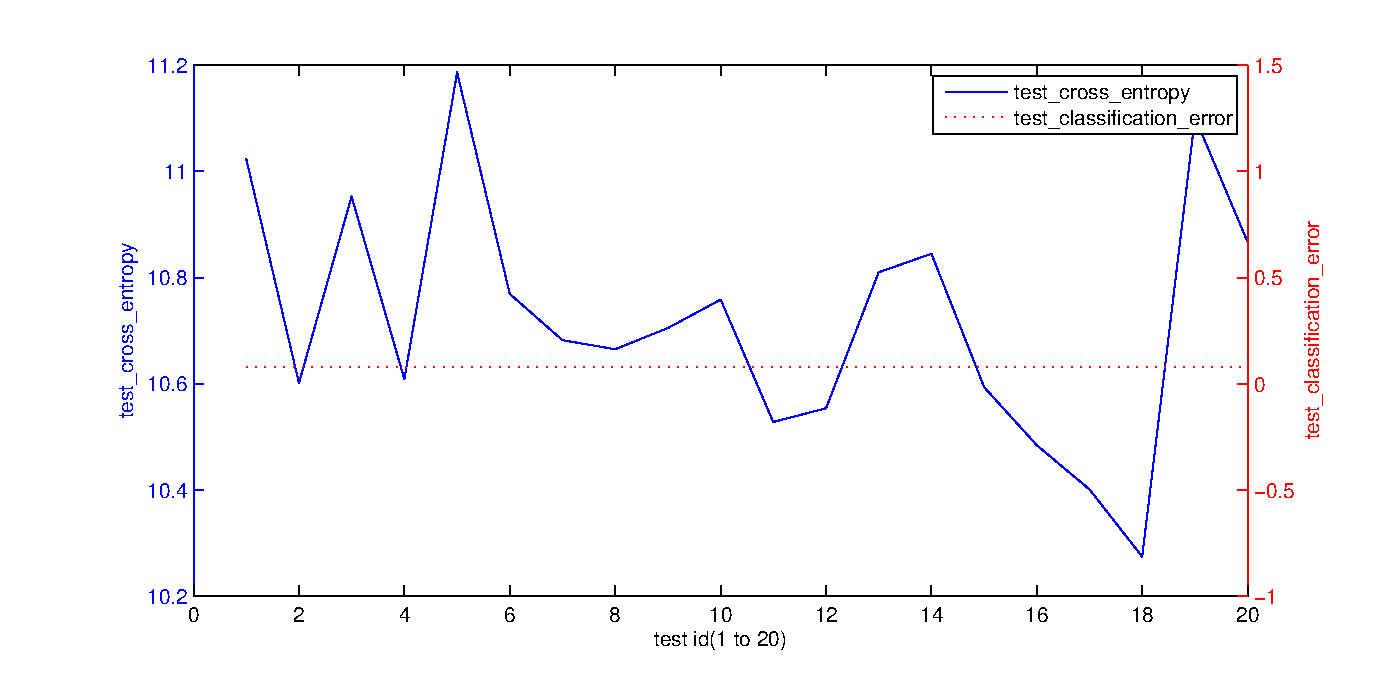
\includegraphics[width=\textwidth]{2-3-test.eps}
\caption{The cross entropy and classification error on the test set over multiple re-runs.
\label{fig:2-3-test}}
\end{figure}

\begin{table}[htbp]
\centering
\begin{tabular}{lcc}
\toprule
$\lambda$ & cross\_entropy(test) & classification\_error(test) \\
\midrule
0.5 & 11.89 & 0.080\\
\bottomrule
\end{tabular}
\caption{The averaged cross entropy and classification error on the test set. 
\label{table:test-final}}
\end{table}

Comparing the results with penalty (Table \ref{table:test-final}) to those without penalty (Table \ref{table:hyper-final}), the cross entropy decreased from 13.95 to 11.89 while the classification error increased from 0.073 to 0.080. \\

So the results with penalty performs a little better, because it can avoid large weights and overfitting. I think we can get better performance if we train and validate with more values of $\lambda$. On the other hand, the logistic regression with penalty can be used to avoid large weights, however, since I initialized the weights using the \texttt{randn} function, it is small and normalized. So if I change another initialization method, the penalty will be more useful.\\

\begin{figure}[htb]
\centering
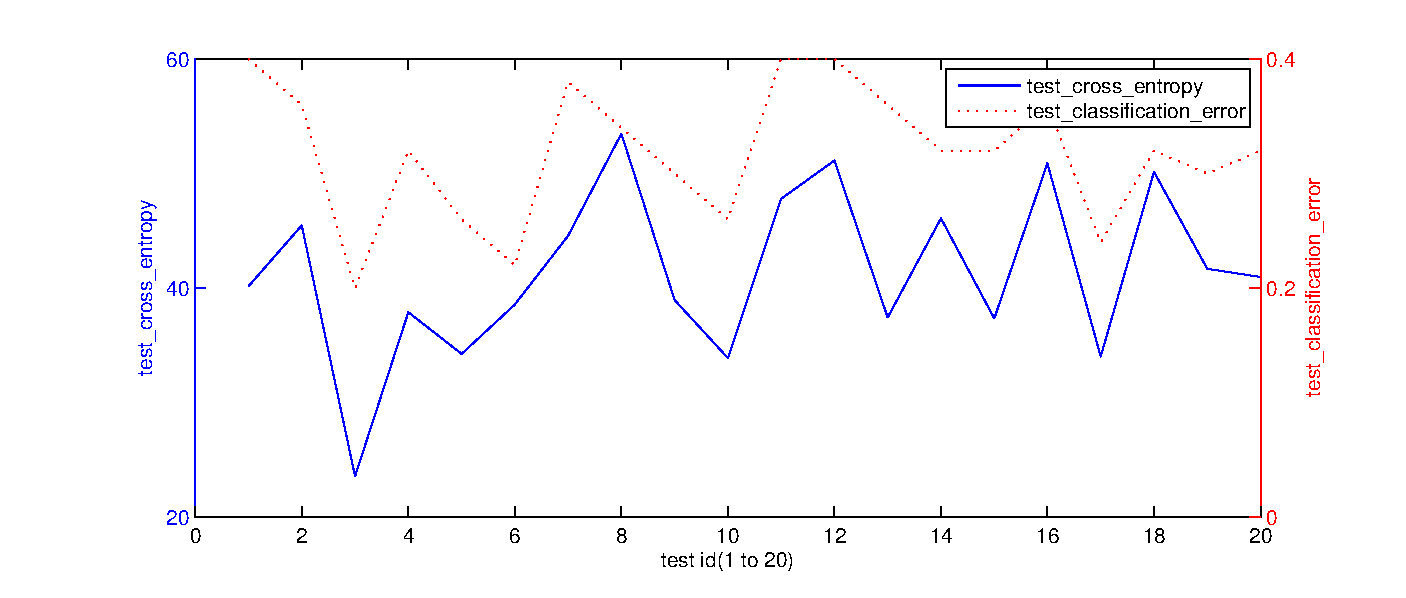
\includegraphics[width=\textwidth]{2-3-test-s.eps}
\caption{The cross entropy and classification error on the test set (trained with \texttt{mnist\_train\_small}) over multiple re-runs.
\label{fig:2-3-test-s}}
\end{figure}

\begin{table}[htbp]
\centering
\begin{tabular}{lcc}
\toprule
$\lambda$ & cross\_entropy(test) & classification\_error(test) \\
\midrule
0.5 & 41.41 & 0.319\\
\bottomrule
\end{tabular}
\caption{The averaged cross entropy and classification error (trained with \texttt{mnist\_train\_small}) on the test set. 
\label{table:test-final-s}}
\end{table}

Let's check with the smaller training set(Figure \ref{fig:2-3-test-s} and Table \ref{table:test-final-s}). We can clearly see that the cross entropy and classification error is significantly high if we trained with a smaller dataset. That also implies that we need a larger training set to avoid problems including overfitting.\\

\subsection{Naive Bayes}

\begin{table}[htbp]
\centering
\begin{tabular}{lcc}
\toprule
\ & training & test \\
\midrule
accuracy & 0.8625 & 0.8000\\
\bottomrule
\end{tabular}
\caption{The training and test accuracy using the naive Bayes model. 
\label{table:acc-nb}}
\end{table}

After training with \texttt{train\_nb.m}, the training and test accuracy calculated by \texttt{test\_nb} is reported in the Table \ref{table:acc-nb}.\\

\begin{figure}[htb]
\centering
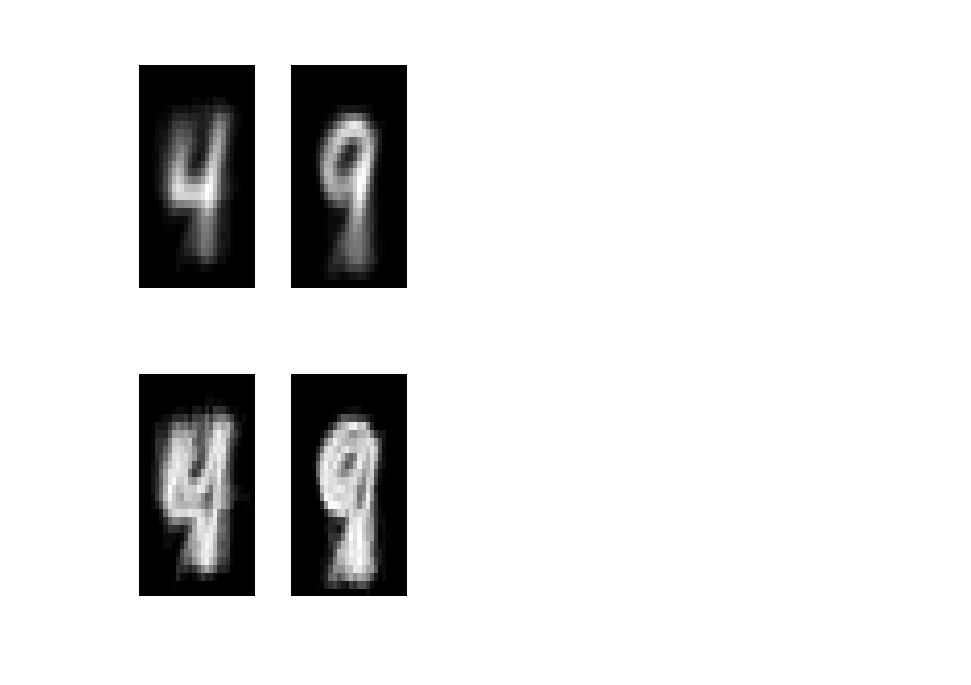
\includegraphics[width=\textwidth]{2-4-digit.eps}
\caption{The visualization of the mean and variance vectors $\mu_c$ and $\sigma_c^2$ for class "4" and "9", generated by \texttt{plot\_digits.m}. The two plots on the 1st line denotes the mean of the model, in which the pixel color represents the average handwriting of the two digits. The other two plots on the 2nd line denotes the variance of the model, in which the bright pixel implies a larger variance.
\label{fig:2-4-digit}}
\end{figure}

The plots of the two digits seems reasonable. The plots imply the average handwriting of the two digits (mean), as well as the difference between the training samples (variance). We can understand clearly about what "4" and "9" look like from the mean plot. We can also observe the fluctuant pixels on the variance plot, which represents the difference of handwriting among the people.\\

The accuracy rate is not perfect, maybe we need to use a more complicated model instead of the Naive Bayes. The assumption of the independent features may not true in this problem, for example, people would rather write a digit continuously other than tap the pixel one by one with a needle. So we need to consider the covariance matrix to improve the accuracy rate.\\

\subsection{Comparison}

\begin{table}[htbp]
\centering
\begin{tabular}{lcccc}
\toprule
\ & $k$-NN & Logistic Regression & Penalized Logistic Regression & Naive Bayes\\
\midrule
accuracy & 0.940 & 0.927 & 0.920 & 0.800\\
\bottomrule
\end{tabular}
\caption{The accuracy of the digit classification task on the test set (trained with \texttt{mnist\_train}) using different models, including $k$-NN, Logistic Regression, Penalized Logistic Regression, and Naive Bayes. 
\label{table:acc-all}}
\end{table}

It seems that $k$-NN performs best, and Naive Bayes performs worse. Then let's observe the results on a smaller training set \texttt{mnist\_train\_small}.\\

\begin{table}[htbp]
\centering
\begin{tabular}{lcccc}
\toprule
\ & $k$-NN & Logistic Regression & Penalized Logistic Regression & Naive Bayes\\
\midrule
accuracy & 0.660 & 0.675 & 0.681 & 0.660\\
\bottomrule
\end{tabular}
\caption{The accuracy of the digit classification task on the test set (trained with \texttt{mnist\_train\_small}) using different models, including $k$-NN, Logistic Regression, Penalized Logistic Regression, and Naive Bayes. 
\label{table:acc-s-all}}
\end{table}

This time the Penalized Logistic Regression seems to perform better, while $k$-NN became the worst. It can be implied that $k$-NN and Naive Bayes need more training data to get good performance. Of course the other methods also need lots of training data. This is what people do in practical: find more data, and train.\\

\end{document}